\qs{}{
    How many courses do each professor handle?
}

This counts uniquely the courses they handle, which are grouped according to the professor's name from the course table.
\vspace{\baselineskip}

\sol{}
\noindent\line(1, 0){0.89\linewidth}
\begin{verbatim}
SELECT crs_instr AS "Professor Name", COUNT(DISTINCT crs_code) AS "No. of Courses Handled"
FROM course
GROUP BY crs_instr;
\end{verbatim}
\noindent\line(1, 0){\linewidth}

\begin{figure}[H]
    \centering
    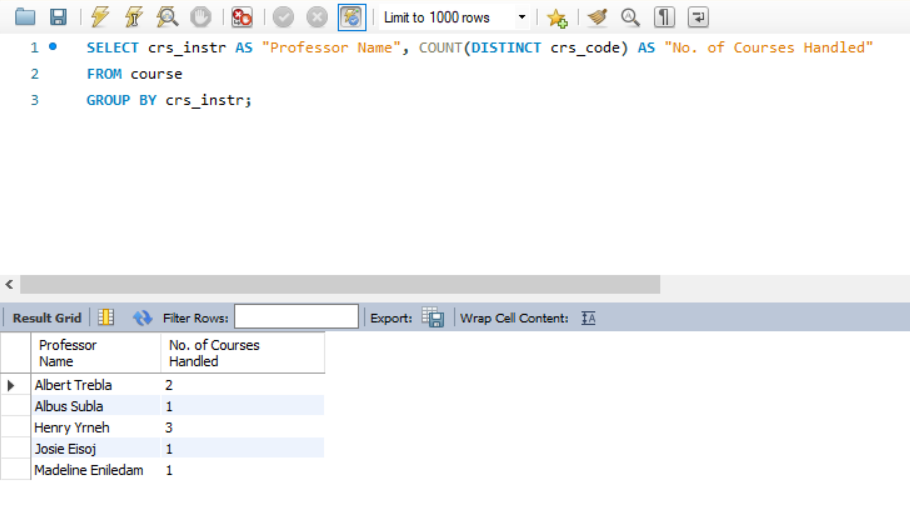
\includegraphics[width=0.7\linewidth]{images/q11.png}
    \caption{Question 11 Query and Output}
\end{figure}
